% !TeX spellcheck = de_DE
\chapter{Grundlagen digitaler Signalverarbeitung in Hörgeräten}
\label{chap:grundlagen}
In diesem Kapitel wird kurz auf die Grundlagen und Begriffe von Signalprozessoren anhand der zugrundeliegenden Architektur eingegangen. Im Anschluss werden einzelne für diese Arbeit relevante Bestandteile genauer beschrieben. Darauf hin soll ein kurzer Einblick in verwandte Ansätze gegeben werden um im weiteren Verlauf die Funktion des Scheduling und das Prinzip der Verlustleistung zu beschreiben. Das Ende des Kapitels gibt eine grobe Übersicht über Genetische-Algorithmen gegeben.

%\section{FPGA}
%Bei einem FPGA (Field Programmable Gate Array) handelt es sich um ein frei programmierbaren integrierten Schaltkreis, welcher mithilfe von Look-Up-Tabellen sehr effizient Algorithmen abbildet. Um eine gewünschte Funktion auf dem FPGA zu implementieren ist es notwendig die Look-Up-Tabellen mit einer Wahrheitstabellen zu befüllen, welche diese Funktion abbildet. Dadurch kann ein FPGA jegliche erdenkliche Aufgabe erfüllen. Um die beschriebenen Blöcke mit dem IO-Ports des Chips zu verbinden ist es notwendig eine Verbindung mithilfe von Rooting-Switches und Connection-Boxen zu erstellen. Damit der Chip konfiguriert werden kann, muss die Funktion mithilfe einer HDL(Hardware Description Language) beschrieben werden.\cite{farooq2012fpga} Vorteil dieser Implementierung ist, dass eine echte Parallelität erreicht werden kann, so dass mehrere Blöcke zeitgleich ausführbar sind. In dieser Arbeit wird ein FPGA als Entwicklungsumgebung verwendet, um den zu entwickelnden ASIP bestmöglich abzubilden und dabei möglichst flexibel zu bleiben.


%\section{ASIP}
%ASIP ist die Abkürzung für Application Specific Instruction Set Processor. Die Architektur dieses Prozessors ist anwendungsspezifisch optimiert. Hierbei sind ASIPs meist auf eine gewisse Funktion optimiert. Durch diese Spezialisierung, ist es möglich Einsparungen hinsichtlich Siliziumfläche und Energieverbrauch gegenüber herkömmlichen Prozessoren zu erreichen. Der in dieser Arbeit verwendete ASIP ist eine vereinfachte Variante eines MIPS-Prozessors. MIPS oder auch \glqq Microprocessor without interlocked pipeline stages\grqq{} ist eine Befehlssatzarchitektur bei der der Entwickler/Compiler, Datenabhängigkeiten der Befehle erkennen und auflösen muss.

%\section{SIMD}
%\label{sec:SIMD}
%Der Begriff SIMD steht für Single Instruction Multiple Data und ist eine Datenverarbeitungseigenschaft von Prozessoren, die meist in der Signalverarbeitung zum Einsatz kommt. Der Vorteil einer solchen Implementierung ist, dass eine Instruktion in mehreren ALUs parallel, mit unterschiedlichen Daten ausgeführt werden kann. Somit ist nur eine Instruktion für die Berechnung vieler Operationen nötig, dadurch ist eine erhebliche Performanz-Steigerung erreichbar.\cite[Seite 249]{wust2010mikroprozessortechnik}

%\subsection{VLIW}
%\label{sec:VLIW}
%VLIW ist eine Eigenschaft von Mikroprozessor-Architekturen. VLIW steht hierbei für Very Long Instruction Word und bedeutet soviel wie sehr langes Instruktions-Wort. Das Ziel dieser Struktur ist eine schnelle Abarbeitung des Befehlsatzes, wobei hierbei einige Befehle parallel ausgeführt werden können. Um dies zu ermöglichen sind mehrere Instruktions-Dekoder vonnöten. Eine VLIW-Architekur geht meist mit Pipelining einher. 

%\subsection{Pipelining}
%Wie das Wort Pipelining schon besagt, handelt es sich hierbei um eine Befehlsabarbeitung am Fließband(Pipeline). Wurde ein Befehl in der ersten Pipelinestufe abgearbeitet kann dieser an die nächste Stufe weitergeleitet werden und der nachfolgende Befehl führt die erste Stufe aus. Die Zeit bis ein Befehl alle Piplinestufen passiert hat nennt man Latenzzeit und dauert genau so viele Takte wie die Pipeline Stufen hat.(siehe Abbildung \ref{fig:pipeline}) Diese Verzoegerung macht ist jedoch nur beim Befüllen der Pipeline bemerktbar, im Idealfall kann im Anschluss mit jedem Takt ein Befehl beendet werden. Somit ist eine parallele Verarbeitung mehrerer unterschiedlicher Befehle möglich. Dabei ist darauf zu achten, dass die Taktung der Pipelinestufen sich an der Stufe orientiert, welcher die längste Ausführungsdauer aufweist. \cite[Seite 204]{wust2010mikroprozessortechnik}
%\begin{scriptsize}
%	\begin{figure}[htbp] 
%		\centering
%		\includesvg[width=0.70\textwidth]{pipeline}
%		\caption{Pipeline-Prinzip}
%		\label{fig:pipeline}
%	\end{figure}
%\end{scriptsize}

\section{Aufbau der Architektur}
\label{chap:architecture_overview}
Bei dem verwendeten Prozessor handelt es sich um ein MIPS-Prozessor der Teil des RAPANUI Projektes ist. Es handelt sich hierbei um ein ASIP-Prozessor. ASIP ist die Abkürzung für Application Specific Instruction Set Processor. Die Architektur dieses Prozessors ist anwendungsspezifisch optimiert. Hierbei sind ASIPs meist auf eine gewisse Funktion optimiert. Durch diese Spezialisierung, ist es möglich Einsparungen hinsichtlich Siliziumfläche und Energieverbrauch gegenüber herkömmlichen Prozessoren zu erreichen. MIPS oder auch \glqq Microprocessor without interlocked pipeline stages\grqq{} ist eine Befehlssatzarchitektur bei der der Entwickler/Compiler, Datenabhängigkeiten der Befehle erkennen und auflösen muss.
Um dem niedrigen Energieverbrauch und Flächenbedarf bei Hörgeräten zu genügen, handelt es sich bei dem Prozessor zusätzlich um eine vereinfacht Implementierung der MOAI-Prozessor-Architektur(siehe Abbildung \ref{fig:KAVUAKA}). Dieser wird auch KAVUAKA genannt und ist ein VLIW-SIMD ASIP Prozessor.\\
Bei VLIW  handelt es sich hierbei um eine Eigenschaft von Mikroprozessor-Architekturen. VLIW steht für Very Long Instruction Word und bedeutet soviel wie sehr langes Instruktions-Wort. Das Ziel dieser Struktur ist eine schnelle Abarbeitung des Befehlsatzes, wobei hierbei einige Befehle parallel ausgeführt werden können. Um dies zu ermöglichen sind mehrere Instruktions-Dekoder vonnöten. Eine VLIW-Architekur geht meist mit Pipelining einher.\\
Der Begriff SIMD steht für Single Instruction Multiple Data und ist eine Datenverarbeitungseigenschaft von Prozessoren, die meist in der Signalverarbeitung zum Einsatz kommt. Der Vorteil einer solchen Implementierung ist, dass eine Instruktion in mehreren ALUs parallel, mit unterschiedlichen Daten ausgeführt werden kann. Somit ist nur eine Instruktion für die Berechnung vieler Operationen nötig, dadurch ist eine erhebliche Performanz-Steigerung erreichbar.\cite[Seite 249]{wust2010mikroprozessortechnik}\\
Außerdem verfügt die Architektur des verwendeten Prozessors über zwei Pipeline-Stufen.
Wie das Wort Pipelining schon besagt, handelt es sich hierbei um eine Befehlsabarbeitung am Fließband(Pipeline). Wurde ein Befehl in der ersten Pipelinestufe abgearbeitet kann dieser an die nächste Stufe weitergeleitet werden und der nachfolgende Befehl führt die erste Stufe aus. Die Zeit bis ein Befehl alle Piplinestufen passiert hat nennt man Latenzzeit und dauert genau so viele Takte wie die Pipeline Stufen hat.(siehe Abbildung \ref{fig:pipeline}) Diese Verzögerung mach sich jedoch nur beim Befüllen der Pipeline bemerkbar, im Idealfall kann im Anschluss mit jedem Takt ein Befehl beendet werden. Somit ist eine parallele Verarbeitung mehrerer unterschiedlicher Befehle möglich. Dabei ist darauf zu achten, dass die Taktung der Pipelinestufen sich an der Stufe orientiert, welcher die längste Ausführungsdauer aufweist. \cite[Seite 204]{wust2010mikroprozessortechnik}
\newpage
\begin{scriptsize}
	\begin{figure}[htbp] 
		\centering
		\includesvg[width=0.70\textwidth]{pipeline}
		\caption{Pipeline-Prinzip}
		\label{fig:pipeline}
	\end{figure}
\end{scriptsize}

Die beiden Pipelinestufen des verwendeten KUAVAKA-Prozessors sind wie folgt aufgeteilt:
\begin{itemize}
	\item[1.] Instruction Fetch - Decode - Register Access (IF - DE - RA) 
	\item[2.] Execute - Write Back (EX - WB)
\end{itemize}

Des weiteren wurde der Prozessor so erweitert, dass neue Funktionen sowie Co-Prozessoren eingefügt werden können. Zudem besteht die Möglichkeit des Forwarding bei der Verwendung von temporären Variablen.
Der verwendete KAVUAKA-Prozessor besitzt außerdem zwei Instruktion-Dekoder auch Issue-Slots genannt und kann somit zwei Befehle parallel ausführen.
Fuer die Implementierung wird der Prozessor auf einem ASIC entwickelt und zur Verifikation auf einem FPGA getestet, da dieser eine hohe Flexibilität, sowie geringere Entwicklungszeiten bietet und die spätere Hardware eins zu eins Abgebildet werden kann.\cite{lukasglitches2017}
Bei ASICs handelt sich um anwendungsspezifische Schaltungen die in einer Integrierten Schaltung zusammengefuegt werden, hierbei ist die komplette Funktion in Hardware abgebildet und ist somit äußerst klein in der Bauweise, performant und gleichzeitig energie-effizient. 

\begin{scriptsize}
	\begin{figure}[htbp] 
		\centering
		\includesvg[width=0.70\textwidth]{kavuaka2pipeline}
		\caption[KAVUAKA-Prozessor]{KAVUAKA-Prozessor \cite{lukasglitches2017}}
		\label{fig:KAVUAKA}
	\end{figure}
\end{scriptsize}


\subsection{Register File Organisation}
Es besteht eine Vielzahl an Registerorganisationen für Signalprozessoren. Im Allgemeinen lassen sich diese auf vier Grundorganisationen herunterbrechen: zentralisierte, gruppierte, hierarchische und partitionierte Registerorganisation (siehe Abbildung \ref{fig:RegisterOrga}).\newline
\begin{figure}[htbp] 
	\centering
	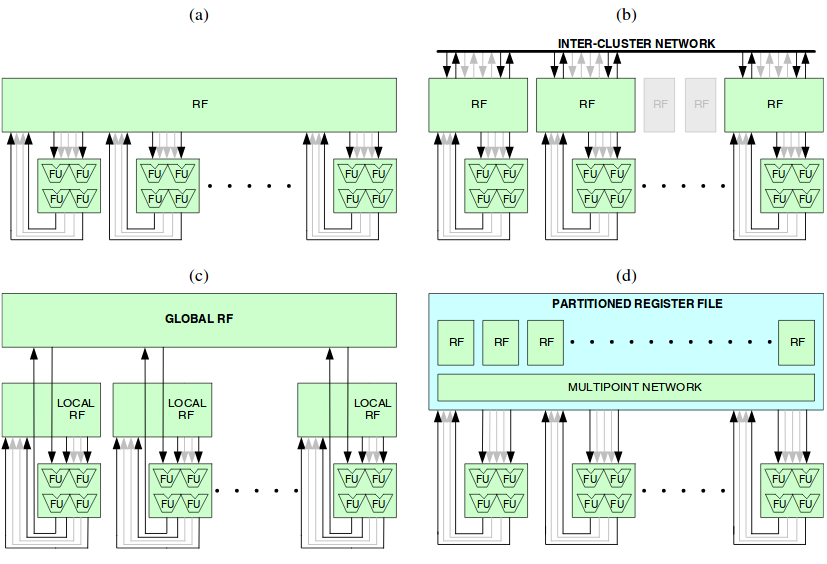
\includegraphics[width=\textwidth]{fig/Register_orga.png}
	\caption[Register File Organisation]{Register File Organisation –\\ a)zentralisierte Organisation b)gruppierte Organisation c)hierarchische Organisation d)partitionierte Organisation  \cite{paya2010multi}}
	\label{fig:RegisterOrga}
\end{figure}
\newline
Im folgenden soll nun weiter auf die partitionierte Organisation eingegangen werden. Physikalisch ist der Prozessor mit einem 4kB Register File ausgestattet. Dabei handelt es sich nicht um eine monolithische sondern um ein Multishared Register-File Organisation. Hierbei wird das Register in mehrere Teile getrennt, die Anzahl hängt hierbei von den Issue-Solts ab. Durch diese Aufteilung können Einsparungen in der Logik für die Schreib- und Leseports generiert werden und die Anzahl der Register-File-Ports wird erhöht.\\
Der verwendete Prozessor besitzt zwei Register-Files mit jeweils 32 64bit-Registern. Beide Register weisen zwei Lese und vier Schreibports auf. Dadurch ist es möglich, dass Instruktionen aus dem Issue-Slot 1 in das Register-File 0 schreiben oder lesen und umgekehrt. Außerdem wird durch diese Architektur ein Schreiben und Lesen zweier Instruktionen auf das selbe Register-File möglich gemacht. Des weiteren können im Falle einer X2-Instruktion beide Ports des Registers verwendet werden. Die Aufteilung und  Zuordnung der Schreib- und Leseports können aus der Abbildung \ref{fig:reg_orga} und \ref{fig::schreib-port}+\ref{lese-port} entnommen werden.


%\begin{figure}[htbp] 
%	\centering
%	\includesvg[width=0.7\textwidth]{registerfile_new}
%	\caption{Register File Organistaion}
%	\label{fig:reg_orga}
%\end{figure}

\begin{table}[htbp]
	
	\begin{minipage}{.5\textwidth}
		\flushleft
		\begin{tabular}{cccccc}
			\multicolumn{2}{l}{Write-Ports}                 & \multicolumn{4}{|l}{Register-Ports}                                                               \\ 
			\multicolumn{1}{c}{0} & \multicolumn{1}{c}{1} & \multicolumn{1}{|c}{0} & \multicolumn{1}{c}{1} & \multicolumn{1}{c}{2} & \multicolumn{1}{c}{3} \\ 
			\hline
			\multicolumn{1}{c}{0} & \multicolumn{1}{c}{0} & \multicolumn{1}{|c}{0} & \multicolumn{1}{c}{1} & \multicolumn{1}{c}{} & \multicolumn{1}{c}{} \\ 
			\multicolumn{1}{c}{0} & \multicolumn{1}{c}{1} & \multicolumn{1}{|c}{0} & \multicolumn{1}{c}{} & \multicolumn{1}{c}{1} & \multicolumn{1}{c}{} \\ 
			\multicolumn{1}{c}{1} & \multicolumn{1}{c}{0} & \multicolumn{1}{|c}{1} & \multicolumn{1}{c}{} & \multicolumn{1}{c}{0} & \multicolumn{1}{c}{} \\ 
			\multicolumn{1}{c}{1} & \multicolumn{1}{c}{1} & \multicolumn{1}{|c}{} & \multicolumn{1}{c}{} & \multicolumn{1}{c}{0} &  \multicolumn{1}{c}{1}                   
		\end{tabular}
		\caption{\label{fig::schreib-port}Schreib-Port}
	\end{minipage}
	\hfill
	\begin{minipage}{.5\textwidth}
		\flushleft
		
		\begin{tabular}{cccccccccccccccccc}
			\multicolumn{4}{l}{Read-Ports.}                 & \multicolumn{8}{|l}{Register-Ports}                                                               \\ 
			\multicolumn{1}{c}{0} & \multicolumn{1}{c}{1} & \multicolumn{1}{c}{2} & \multicolumn{1}{c}{3} & \multicolumn{1}{|c}{0} & \multicolumn{1}{c}{1} & \multicolumn{1}{c}{2}& \multicolumn{1}{c}{3} &
			\multicolumn{1}{c}{4} & \multicolumn{1}{c}{5} & \multicolumn{1}{c}{6}& \multicolumn{1}{c}{7} \\
			\hline
			\multicolumn{1}{c}{0} & \multicolumn{1}{c}{0} & \multicolumn{1}{c}{0} & \multicolumn{1}{c}{0} & \multicolumn{1}{|c}{0} & \multicolumn{1}{c}{1} & \multicolumn{1}{c}{2}& \multicolumn{1}{c}{3} &
			\multicolumn{1}{c}{} & \multicolumn{1}{c}{} & \multicolumn{1}{c}{}& \multicolumn{1}{c}{} \\
			\multicolumn{1}{c}{0} & \multicolumn{1}{c}{0} & \multicolumn{1}{c}{0} & \multicolumn{1}{c}{1} & \multicolumn{1}{|c}{0} & \multicolumn{1}{c}{1} & \multicolumn{1}{c}{2}& \multicolumn{1}{c}{} &
			\multicolumn{1}{c}{3} & \multicolumn{1}{c}{} & \multicolumn{1}{c}{}& \multicolumn{1}{c}{} \\
			\multicolumn{1}{c}{0} & \multicolumn{1}{c}{0} & \multicolumn{1}{c}{1} & \multicolumn{1}{c}{0} & \multicolumn{1}{|c}{0} & \multicolumn{1}{c}{1} & \multicolumn{1}{c}{3}& \multicolumn{1}{c}{} &
			\multicolumn{1}{c}{2} & \multicolumn{1}{c}{} & \multicolumn{1}{c}{}& \multicolumn{1}{c}{} \\
			\multicolumn{1}{c}{0} & \multicolumn{1}{c}{0} & \multicolumn{1}{c}{1} & \multicolumn{1}{c}{1} & \multicolumn{1}{|c}{0} & \multicolumn{1}{c}{1} & \multicolumn{1}{c}{}& \multicolumn{1}{c}{} &
			\multicolumn{1}{c}{3} & \multicolumn{1}{c}{2} & \multicolumn{1}{c}{}& \multicolumn{1}{c}{} \\
			\multicolumn{1}{c}{0} & \multicolumn{1}{c}{1} & \multicolumn{1}{c}{0} & \multicolumn{1}{c}{0} & \multicolumn{1}{|c}{0} & \multicolumn{1}{c}{2} & \multicolumn{1}{c}{3}& \multicolumn{1}{c}{} &
			\multicolumn{1}{c}{1} & \multicolumn{1}{c}{} & \multicolumn{1}{c}{}& \multicolumn{1}{c}{} \\
			\multicolumn{1}{c}{0} & \multicolumn{1}{c}{1} & \multicolumn{1}{c}{0} & \multicolumn{1}{c}{1} & \multicolumn{1}{|c}{0} & \multicolumn{1}{c}{2} & \multicolumn{1}{c}{}& \multicolumn{1}{c}{} &
			\multicolumn{1}{c}{3} & \multicolumn{1}{c}{1} & \multicolumn{1}{c}{}& \multicolumn{1}{c}{} \\
			\multicolumn{1}{c}{0} & \multicolumn{1}{c}{1} & \multicolumn{1}{c}{1} & \multicolumn{1}{c}{0} & \multicolumn{1}{|c}{0} & \multicolumn{1}{c}{3} & \multicolumn{1}{c}{}& \multicolumn{1}{c}{} &
			\multicolumn{1}{c}{2} & \multicolumn{1}{c}{1} & \multicolumn{1}{c}{}& \multicolumn{1}{c}{} \\
			\multicolumn{1}{c}{0} & \multicolumn{1}{c}{1} & \multicolumn{1}{c}{1} & \multicolumn{1}{c}{1} & \multicolumn{1}{|c}{0} & \multicolumn{1}{c}{} & \multicolumn{1}{c}{}& \multicolumn{1}{c}{} &
			\multicolumn{1}{c}{3} & \multicolumn{1}{c}{2} & \multicolumn{1}{c}{1}& \multicolumn{1}{c}{} \\
			\multicolumn{1}{c}{1} & \multicolumn{1}{c}{0} & \multicolumn{1}{c}{0} & \multicolumn{1}{c}{0} & \multicolumn{1}{|c}{1} & \multicolumn{1}{c}{2} & \multicolumn{1}{c}{3}& \multicolumn{1}{c}{} &
			\multicolumn{1}{c}{0} & \multicolumn{1}{c}{} & \multicolumn{1}{c}{}& \multicolumn{1}{c}{} \\
			\multicolumn{1}{c}{1} & \multicolumn{1}{c}{0} & \multicolumn{1}{c}{0} & \multicolumn{1}{c}{1} & \multicolumn{1}{|c}{1} & \multicolumn{1}{c}{2} & \multicolumn{1}{c}{}& \multicolumn{1}{c}{} &
			\multicolumn{1}{c}{3} & \multicolumn{1}{c}{0} & \multicolumn{1}{c}{}& \multicolumn{1}{c}{} \\
			\multicolumn{1}{c}{1} & \multicolumn{1}{c}{0} & \multicolumn{1}{c}{1} & \multicolumn{1}{c}{0} & \multicolumn{1}{|c}{1} & \multicolumn{1}{c}{3} & \multicolumn{1}{c}{}& \multicolumn{1}{c}{} &
			\multicolumn{1}{c}{2} & \multicolumn{1}{c}{0} & \multicolumn{1}{c}{}& \multicolumn{1}{c}{} \\
			\multicolumn{1}{c}{1} & \multicolumn{1}{c}{0} & \multicolumn{1}{c}{1} & \multicolumn{1}{c}{1} & \multicolumn{1}{|c}{1} & \multicolumn{1}{c}{} & \multicolumn{1}{c}{}& \multicolumn{1}{c}{} &
			\multicolumn{1}{c}{3} & \multicolumn{1}{c}{2} & \multicolumn{1}{c}{0}& \multicolumn{1}{c}{} \\
			\multicolumn{1}{c}{1} & \multicolumn{1}{c}{1} & \multicolumn{1}{c}{0} & \multicolumn{1}{c}{0} & \multicolumn{1}{|c}{2} & \multicolumn{1}{c}{3} & \multicolumn{1}{c}{}& \multicolumn{1}{c}{} &
			\multicolumn{1}{c}{1} & \multicolumn{1}{c}{0} & \multicolumn{1}{c}{}& \multicolumn{1}{c}{} \\
			\multicolumn{1}{c}{1} & \multicolumn{1}{c}{1} & \multicolumn{1}{c}{0} & \multicolumn{1}{c}{1} & \multicolumn{1}{|c}{2} & \multicolumn{1}{c}{} & \multicolumn{1}{c}{}& \multicolumn{1}{c}{} &
			\multicolumn{1}{c}{3} & \multicolumn{1}{c}{1} & \multicolumn{1}{c}{0}& \multicolumn{1}{c}{} \\
			\multicolumn{1}{c}{1} & \multicolumn{1}{c}{1} & \multicolumn{1}{c}{1} & \multicolumn{1}{c}{0} & \multicolumn{1}{|c}{3} & \multicolumn{1}{c}{} & \multicolumn{1}{c}{}& \multicolumn{1}{c}{} &
			\multicolumn{1}{c}{2} & \multicolumn{1}{c}{1} & \multicolumn{1}{c}{0}& \multicolumn{1}{c}{} \\
			\multicolumn{1}{c}{1} & \multicolumn{1}{c}{1} & \multicolumn{1}{c}{1} & \multicolumn{1}{c}{1} & \multicolumn{1}{|c}{} & \multicolumn{1}{c}{} & \multicolumn{1}{c}{}& \multicolumn{1}{c}{} &
			\multicolumn{1}{c}{3} & \multicolumn{1}{c}{2} & \multicolumn{1}{c}{1}& \multicolumn{1}{c}{0} \\
			
		\end{tabular}
		\caption{\label{lese-port}Lese-Port}
	\end{minipage}
\end{table}


\newpage
\subsection{Optimierungsziel}
In den meisten Prozessoren nimmt das Register-File deutlich mehr als 40\% der gesamten Chipfläche ein. 
Betrachtet man die prozentuale Verteilung der Verlustleistungen, sticht die der Register deutlich hervor. Dadurch ergibt sich ein sehr hohes Optimierungspotential. In dieser Arbeit wird dieses Potential durch einen geeigneten Compiler ausgenutzt. Dabei liegt der Fokus auf der Verlustleistungsoptimierung der Register-Files. Der Vorteil einer Optimierung zur Compilezeit liegt darin, dass keinerlei neue Hardware benötigt wird. Dies macht das es äußerst lukrative. Dabei handelt es sich um kein neuem Ansatz denn bereits...  Haben sich mit diesem Problem befasst und Lösungen gefunden. Die meisten Literaturen befassen sich bei der Optimierung jedoch auf das Scheduling und die Ausführungszeit der Codes. Die Besonderheit bei dem Ansatz in dieser Arbeit liegt bei der Optimierung der Verlustleistung durch den Compiler. Die Hauptkomponenten des Compilers sind das Scheduling und die Register allocation. Im folgenden soll kurz auf die Funktionen des Compilers eingegangen werden. 
\subsection{Compiler}
%Überleitung zu Tradeoff von Flache und Register File allokation.

Damit ein Prozessor eine Programmiersprache (optimal) ausführen kann sind einige Schritte notwendig. Diese sind im Compiler zusammengefasst und werden im folgenden kurz erläutertert.\\
Der Code wird vorerst in so genannte Micro Instructions (MI) gestückelt.  Hierbei ist eine MI eine Anweisung welche der Prozessor in einem Taktzyklus ausführen kann. Durch die Verwendung eines VLIW-Prozessors ist es möglich mehrere Instruktionen parallel auszuführen. Im Falle des KAUVAKA-Prozessors sind dies wie erwähnt zwei Instruktionen. Aus diesem Grund teilt der Compiler nun die MIs in Micro Operation (MO) auf. Diese werden anschließend in so genannte \glqq Straight Line Microcode\grqq{} (SLM) aufgeteilt. Ein SLM ist hierbei so definiert, dass es nur eine Einsprungstelle und Austrittsstelle gibt. Außerdem dürfen sich keine Sprünge und Verzweigungen innerhalb einer SLM befinden.  Dadurch entsteht ein Baum aus SLMs, die im Anschluss einzeln optimiert werden können. Dieses Verfahren ist nötig, da eine Optimierung über alle Instruktionen eine zu hohe Komplexität aufweisen würde. \cite{landskov1980local}
\subsection{Scheduling}
\label{sec:scheduling}
Das Scheduling ist zuständig für die Anordnung der MIs bzw. MOs die sich in einem SLM befinden. Hierbei geht der Algorithmus so vor, dass er die Anordnung sucht welche den geringsten kritischen Pfad aufweist. Hierbei gibt es verschiedene Ansatzmöglichkeiten. Die einfachste Methode ist das List-Scheduling. Bei diesem Verfahren wird bei jedem einfügen eines MOs überprüft, ob eine valide Register-Allokation möglich ist. Können die Register nicht zugeordnet werden, beginnt der Scheduler mit der nächsten MO. Im darauffolgenden Schritt wird nun nochmals versucht die erste MO einzufügen. Dies wird solange wiederholt bis alle MOs zugeordnet sind.\cite{landskov1980local}
Diese Art von Algorithmus findet jedoch nicht immer eine optimale Lösung und ist gerade für große Programme nicht geeignet. Aus diesem Grund kann optional ein genetischer Algorithmus eingesetzt werden, der die Länge des kritischen Pfades einer SLM reduziert.


\section{Register Allokation}
\label{sec:register allok}
\subsection{Virtuelle Register}
\label{sub:virtuelleR}
Bei virtuellen Registern handelt es sich um Register die an beliebiger Stelle im Register-File allokiert werden können, das heißt der Compiler kann selbst entscheiden wo im Registerfile er diese Variable platziert. 
Die Idee hierbei ist es, dem Compiler die Aufgabe zu übergeben ein geeignetes Register auszuwählen. Das Codebeispiel \ref{phyReg} zeigt anhand einer einfachen Addition diese Funktion. Da der Prozessor nicht mit Immediates addieren kann, müssen zwei Hilfsvariablen verwendet werden. In diesem Fall wurden die Register V0R0 und V0R1 gewählt. Mithilfe dieser Register kann der Prozessor nun eine Addition in Zeile drei durchführen. Anschließend wird der Code in den Speicher zurück geschrieben.
\newpage
\renewcommand{\lstlistingname}{Codebeispiel}
\begin{lstlisting}[frame=single, caption={physikalische Register},captionpos=b,label=phyReg]
MVI V0R0 0x100
MVI V0R1 0x101
ADD V0R0 V0R0 V0R1
STORE 0x100 V0R0
\end{lstlisting}
Um nun den Code etwas flexibler zu gestalten, wird  nun dem Compiler überlassen welches Register er benutzt. Die selbe Addition ist in \ref{virtReg} mit virtuellen Registern realisiert. Hierbei wird dem Compiler durch ein  x gekennzeichnet, dass es sich um ein virtuelles Register handelt. Dieser wählt anschließend ein optimales Register aus, so dass sich der Entwickler um diese Aufgabe nicht bemühen muss. Dies hat den Vorteile, dass somit für den Code geeignete/optimale Register ausgewählt werden können. Hierbei wird darauf geachtet, dass beide Register-Files gleich ausgelastete sind und dass es möglich bleibt X2- oder MAC-Befehle (siehe Kapitel \ref{subsec:x2Mode} ff.) allokiert werden können. Außerdem sind die Register in diesem Fall so allokiert, dass die Verlustleistungsaufnahme minimal ist. Wie die Register für eine optimale Verlustleistung ausgewählt werden müssen wird in dieser Arbeit evaluiert und aufgezeigt.

\begin{lstlisting}[frame=single,caption={virtuelle Register},captionpos=b,label=virtReg]
MV VxR0 0x100
MV VxR1 0x101
ADD VxR0 VxR0 VxR1
STORE 0x100 VxR0
\end{lstlisting}
%\subsection{X2 Betriebsmodus}\label{subsec:x2Mode}
%Der X2-Betriebsmodus ermöglicht es identischen Instruktionen mit dem selben Opcode den Registerzugriff zusammenzuführen, wobei sich die Adresse nur im letzten Bit unterscheidet. Dadurch wurde virtuell die Anzahl der Issue-Slots erhöht, ohne dabei die Anzahl der zu decodierenden Anweisungen zu erhöhen. Hierbei wird einem Befehl die doppelte Anzahl an Schreib- und Lese-Registern übergeben, somit steigt die Zahl der Parameter von drei auf sechs. Bei der Auswahl der Registern gibt es die Vorgabe, dass die erste Instruktionen auf gerade Register-Adressen und die zweite auf ungerade Adressen des zugreift. \cite{paya2009instruction}
\subsection{MAC Operationen}\label{subsec:macMode}
Die MAC(Multiply and Accumulate)-Operation führt eine Multiplikation zweier Werte aus und Akkumuliert diese im Anschluss. Werden bei einer n-bit Implementierungen zwei Werte multipliziert, so kann das Resultat eine Bitbreite von 2n aufweisen. Wird nun eine Architektur mit 64-bit Registern verwendet, müssen zwei Register zur Abspeicherung des Ergebnisses herangezogen werden. Dabei sollte es sich um zwei aufeinanderfolgende Register handeln, hierbei können diese im selben oder in einem benachbarten Register-File stammen. Eine weitere Besonderheit der MAC-Operation ist, dass der erste Operand in eine geraden Registe-Adresse liegen muss. Ein Beispiel für eine valide MAC-Allocation stellt das folgende Register-Paar V0R0 und V1R0 dar.
  

\subsection{Dummy-Register}\label{subsec:dummy}
Dummy-Register sind Register die im Register-File implementiert sind, jedoch kann der Lese- und Schreibzugriff zur Laufzeit über ein so genanntes Dummy-Control-Register gesteuert werden. Mit Hilfe dieser Funktion können beispielsweise Hilfsvariablen die nur kurze Zeit existieren nicht an das Register-File zurück geschrieben werden und somit den Energieverbrauch senkt. 

\subsection{Address-Isolation}\label{subsec:add_iso}
Eine weitere Komponente des Prozessors ist die Adress-Isolation. Dabei handelt es sich um eine Funktion, welche die Switching-Aktivität des Register-Files verringert. Hierbei werden die Adressen der Schreib- und Leseports solange in einem Flipflop gespeichert bis eine neue Adresse angelegt wird.\cite{lukasglitches2017}

\subsection{Clock-Gating}\label{subsec:clock-gate}
Das Taktnetz ist bei Prozessoren in der Regel sehr groß, muss eine hohe Last treiben und hat sehr viele Schaltvorgänge, dadurch nimmt dieses meist über 40\% der Gesamtleistung auf. Aus diesem Grund wurde das Clock-Gating entwickelt. Hinter dem Begriff verbirgt sich eine Abschaltung des Clock-Signals in Teilen des Prozessors der nicht genutzt werden. Dadurch lässt sich die Schaltaktivität in vielen Bereichen des Prozessors deutlich minimieren. Das Resultat spiegelt sich in der Leistungsaufnahme wieder, die dabei deutlich sinkt.\cite{donno2003clock} In dieser Arbeit wird bis auf weiteres kein Clock-Gating eingesetzt.

\section{Verlustleistung}
\label{sec:verlustleistung}
Unter Verlustleistung in integrierten Schaltungen versteht man die in den Transistoren umgesetzte Leistung die in Form von Wärme verloren geht.
Hierbei wird in statische \(P_{stat}\) und dynamische Verlustleistung \(P_{dyn}\) unterschieden. \cite[Seite 4 ff.]{flynn2007low}
\subsection{Dynamische Verlustleistung}\label{subsec:dynVerl}
Jedes mal wenn eine Kapazität geladen oder entladen wird, entsteht eine dynamische Verlustleistung\(P_C\). Eine weitere dynamische Verlustleistung\(P_{SC}\) tritt bei den Schaltevorgang von CMOS-Transistoren auf. Diese soll anhand eines CMOS-Inverters nun verdeutlicht werden. Beim Umschalten der Pegel, entsteht eine kurze Zeitspanne in der beide Transistoren eine leitende Verbindung aufweisen. In diesem Fall besteht ein Kurzschlussstrom \(I_{SC}\)zwischen Versorgungsspannung \(V_{DD}\) und Masse \(V_{SS}\). Die dynamische Verlustleistung ist proportional zur Schaltaktivität\(\alpha\) und somit auch zur Taktfrequenz $f$.\cite[Seite 4 ff.]{flynn2007low}
\begin{equation}
P_{dyn} = \alpha  C_L  V_{dd}^{2}  f
\label{eq:dynVerlustleistung}
\end{equation}
\subsection{Statische Verlustleistung}\label{subsec:statVerl}
Sobald die Verlustleistung unabhängig von der Taktrate ist, kann diese als statische \(P_{Stat}\) bezeichnet werden. Dies ist der Fall, wenn aufbaubedingt ein konstanter Strom zwischen\(V_{DD}\) und\(V_{SS}\)besteht. Dieser Strom ist unabhängig von der angelegten Gatespannung. Der dadurch auftretende Strom wird Leakagestrom genannt. Mit immer kleiner werdenden Strukturen wird dieser Strom deutliche bedeutender.\cite[Seite 8]{flynn2007low}

Die gesamte Verlustleistung ist die Summer der drei erwähnten Verluste.
\begin{equation}
\begin{aligned}
P &= P_{ C }+P_{ SC }+P_{ Stat}\\
P &= P_{dyn}+P_{Stat}
\label{eq:verlustleistung}
\end{aligned}
\end{equation}

\section{Genetische Algorithmen}
\label{sec:genetischer_algo}
Genetische Algorithmen wurden ursprünglich entwickelt um evolutionäre Prozesse aus der Natur nachzuempfinden. Erstmals wurde diese Art von Algorithmen von John Holland 1975 entwickelt und untersucht.
In der Natur müssen sich Lebewesen ständig an ihren Lebensraum anpassen und mit den Problemen der Natur leben. Um dies zu ermöglichen haben sich Lebewesen über Jahrtausende an ihre Umgebungen angepasst. Der Aufbau, die Fähigkeiten und das Erscheinungsbild eines Lebewesen ist von Geburt an vorgegeben, diese Information befindet sich in den Chromosomen verschlüsselt. Eine Evolution ist hierbei die Weitergabe dieser Informationen. Durch das decodieren der Chromosomen entsteht eine neue Lebensform.
Natürliche Selektion ist hierbei die Anpassungsfähigkeit des Lebewesens an den vorgegebenen Lebensraum. Demzufolge überleben bzw. pflanzen sich nur die Generationen fort, welche sich gut an die Umstände der Umgebung angepasst haben. Die Mechanismen hinter der Evolution sind noch nicht komplett entschlüsselt, jedoch sind einige Verfahren bekannt welche im weiteren betrachtet werden.
Durch das Vorbild der Natur sollen mit genetischen Algorithmen schwierige Sachverhalte lösen können. Hierbei stellen die Chromosomen eine Abbildung einer Lösung auf ein Problem dar. Durch eine sogenannte Fitness-Funktion, kann ermittelt werden wie gut sich ein Chromosom an das gegebene Problem angepasst hat. Wie auch in der Natur werden einzelne Chromosomen fortgepflanzt und bilden neue Generationen. Betrachtet man eine gewisse Anzahl an Generationen so spricht man von einer Population. Zu Beginn des Algorithmus startet man mit zufälligen Chromosomen, bis eine bestimmte Anzahl Generationen entstanden ist. Mit dieser Population kann nun die Fortpflanzung betrieben werden.
Durch die Fortpflanzung werden die Chromosomen zweier Lebewesen an eine neue Generation weitergegeben, auch dieser Prozess ist bis heute nicht genau entschlüsselt jedoch können einige Merkmale abgebildet werden. Darunter fällt das Crossover und die Mutation.\cite{davis1991handbook}

\subsection{Fitness}
Die Fitness einer Generation gibt an wie gut sich das Chromosom an das gegebene Problem angepasst hat. Diese Bewertung ist sehr wichtig für die richtige Funktion des Algorithmus. Dabei muss die Fitness-Funktion so entwickelt werden, dass die Generationen unterscheidbar sind und eine Einordnung in der Population möglich ist. 

\subsection{Crossover}
\label{chap:grundlagen_cossover}
Bei dem Crossover-Prozess, handelt es sich um die Fortpflanzung von Generationen. Hierbei ist ausschlaggebend welche Generationen miteinander gepaart werden. Auf den ersten Blick scheint es einleuchtend immer die Generation mit der besten Fitness zu paaren. Dies ist jedoch nicht immer sinnvoll, da so schnell ein lokales Minimum erreicht wird. Aus diesem Grund gibt es verschiedene Ansätze um geeignete Eltern für die neue Generation zu finden.\cite{davis1991handbook} Die am weitesten verbreitete Methode ist die Roulette Wheel Selection. Hierbei wird zufällig ein Elternpaar gewählt, wobei die Chance einer jeden Generation ausgewählt zu werden proportional zur Fitness ist. Dieses Verfahren trägt ihren Namen daher, dass es einem Roulette-Rad gleicht, wobei das Rad in Stücke unterteilt ist, welche die Größe proportional zur Fitness haben. Die Auswahl kann nun einem Drehen an einem Rad gleichgesetzt werden. Hierbei ist es wahrscheinlicher, dass die Generationen mit höher Fitness ausgewählt werden. Es ist jedoch auch möglich, dass Populationsmitglieder mit niedriger Fitness gepaart werden.

\subsection{Mutation}
Auch der Prozess der Mutation stammt aus der Natur. Hierbei besteht eine geringe Chance, dass Chromosomen verändert werden und Eigenschaften aufweisen die in keinem der Elternteile aufzufinden sind. Hierzu werden in dem durch Crossover erzeugtem Chromosom einzelne Gene durch Zufall verändert. Die Wahrscheinlichkeit einer zufälligen Veränderung ist hierbei wie in der Natur sehr gering.\cite{davis1991handbook}

